

\documentclass{sig-alternate-05-2015}

% Include useful packages
\usepackage{graphicx}
\graphicspath{ {images/} }
\usepackage{float}


\begin{document}

% Copyright
\setcopyright{acmcopyright}


\title{A Reimplementation of Online Tracking by Learning Discriminative Saliency Map with Convolutional Neural Network}

\numberofauthors{2} 
\author{
% You can go ahead and credit any number of authors here,
% e.g. one 'row of three' or two rows (consisting of one row of three
% and a second row of one, two or three).
%
% The command \alignauthor (no curly braces needed) should
% precede each author name, affiliation/snail-mail address and
% e-mail address. Additionally, tag each line of
% affiliation/address with \affaddr, and tag the
% e-mail address with \email.
%
% 1st. author
\alignauthor
Aaron Gonzales\\
       \email{gonza647@msu.edu}
% 2nd. author
\alignauthor
Steven MW Hoffman \\
       \email{hoffm470@msu.edu}
}
% There's nothing stopping you putting the seventh, eighth, etc.
% author on the opening page (as the 'third row') but we ask,
% for aesthetic reasons that you place these 'additional authors'
% in the \additional authors block, viz.
\date{19 February 2016}
% Just remember to make sure that the TOTAL number of authors
% is the number that will appear on the first page PLUS the
% number that will appear in the \additionalauthors section.

\maketitle

\begin{figure*}[t]
\centering
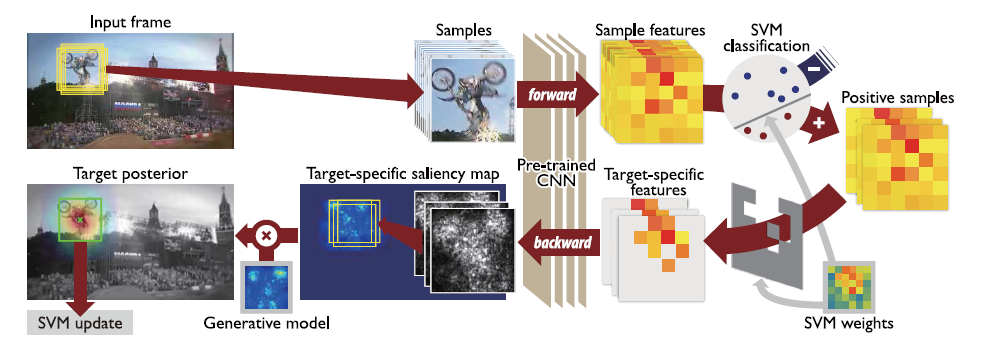
\includegraphics[width=\textwidth]{algorithm}
\caption{A pictoral description of the algorithm described by Hong, et al. in \cite{hong2015online}}
\label{fig:algor}
\end{figure*}

\section{Problem Description}
We chose to implement our machine learning project with a \textit{deep learning thrust}.
We are basing our project on the work of Hong, et al. \cite{hong2015online}, and our goal is to reproduce their work through the creation of a viable demo.
Hong, et al. propose a novel online tracking scheme that is meant for use in applications where tracking an object through frames of a video is desired.
Although there are a large range of potential applications for object tracking software, it is still a difficult problem due to challenges of occlusion, pose variations, illumination changes, fast motion, and background clutter \cite{hong2015online}.
This paper proposes to solve these problems using the combined utility of both a convolutional neural network (CNN) and support vector machine (SVM), wherein a discriminative saliency map is produced and used to calculate the target posterior probability.
The algorithm which they used to achieve this object tracking is described below and is portrayed in Figure \ref{fig:algor}.

The tracking algorithm proposed by \cite{hong2015online} begins by first generating a set of sample images, each of which is drawn from candidate bounding boxes near where the target was located in the previous frame.
Each of these sample images is passed through a pre-trained CNN which was obtained from the Caffe Model Zoo \cite{jia2014caffe}.
A CNN is used because CNNs have been shown to be very successful at creating image representations useful for object discrimination.
For each image, the output from \textit{the first fully-connected layer} of the network is extracted and is used as the feature vector describing that image sample.
The image sample feature vector is then given to an SVM which will classify it as either a positive sample, including the object we are tracking, or a negative sample, which does not include the object we are tracking.
In contrast to the CNN, which is learned offline on generic image data not specific to the target, the SVM is learned online using all the positive samples it has seen until the previous time step.
This allows the SVM to adapt to different types of objects which the user would like to track.
For each positive sample, the target-specific features are extracted by using those features which corresponded to positive weights in the SVM, setting all other feature values to zero.
These target-specific features are then backpropagated through the CNN, producing an image containing a saliency map.
A saliency map is created for every positive sample, and these are combined to make a final target-specific saliency map where larger values in the map indicate a larger posterior probability that the target is located at that pixel.
Through this means, the target can be segmented out of the image at a near pixel level.
With the target successfully segmented out of the frame, the algorithm begins a new in the next frame, creating candidate bounding boxes around where it found the target in the previous frame.

\section{Related Work}
The problem of object tracking in video is a large domain, so we will restrict our discussion here to a few works which also attempted to use CNNs to perform tracking, as these are most relevant to the paper we have chosen by Hong, et al. \cite{hong2015online}.
We also highlight how the approach proposed by Hong, et al. differs from these approaches, making it a novel work.

\cite{fan2010human} utilizes a CNN for tracking; however they use an offline trained CNN. They also require a separate class-specific network to track various other objects. Hong, et al \cite{hong2015online}, in contrast, proposes using a pre-trained CNN used for large scale image classification which is trained on generic image data. An online trained SVM is then used in conjunction with the CNN by Hong, et al. to learn the target specific information.

\cite{NIPS2013_5192} also uses a pre-trained network where a stacked denoising autoencoder is trained using a large number of images to learn generic image features. However, as this network is trained on small grey images, its representation power is limited.

\cite{7362006} proposed a target-specific CNN for tracking, where the CNN is trained online. However, this network is shallow in comparison with the deep CNN proposed by \cite{hong2015online}, and as such does not take advantage of the rich information a deep CNN provides.

In addition to the novelties described above, the tracking method proposed by \cite{hong2015online} differs from all three of the above papers in a few important ways.
First, it uses an online trained SVM with the offline trained CNN in order to adapt the tracking to whatever type of object the algorithm happens to be presented with.
Secondly, it uses saliency maps to find the precise location of the tracked object.

\begin{figure*}[t]
\centering
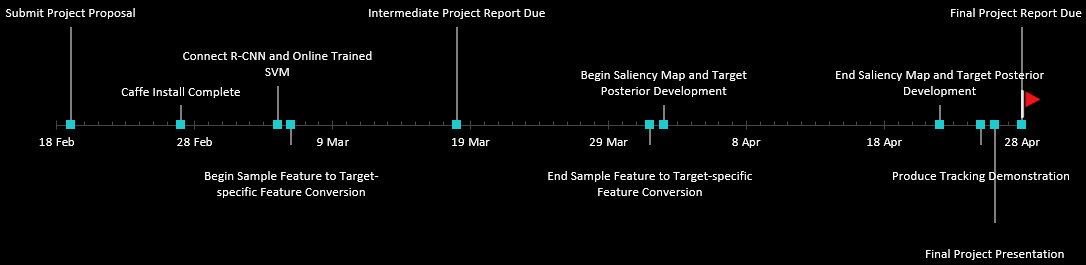
\includegraphics[width=\textwidth]{ProposedTimeline}
\caption{Our project milestones with tentative completion dates. Each tick-mark represents one day on the timeline.}
\label{fig:milestones}
\end{figure*}

\section{Project Milestones}
Featured in Figure \ref{fig:milestones} is our proposed milestone timeline. We anticipate that our Caffe installation will not be complete on our server until late next week. While we await its completion, our goal will be to find a suitable online trained SVM to connect to our R-CNN and to download the object tracking dataset mentioned by \cite{hong2015online}. This may not take as long as represented by the timeline, but we want to ensure we allow ourselves sufficient time to account for any circumstances that may delay our progress. Immediately after having found our R-CNN and SVM, we will begin the process of converting sample features to target-specific features. We anticipate this will take a large swathe of time, and represent that accordingly on our timeline - once this is complete we will begin the end stage our project by developing the saliency maps and calculating the target posterior. A rough outline of the tracking process is provided in Figure \ref{fig:algor}, and may make the proposed milestones more understandable. We would like to provide a demo of our implemented tracking algorithm as well, and so this is our final milestone.
\bibliography{proj-proposal}
\bibliographystyle{unsrt}
\end{document}
